\documentclass[tikz,border=8pt]{standalone}
\usepackage{amsmath,amssymb,lmodern}
\usetikzlibrary{arrows.meta}
\begin{document}
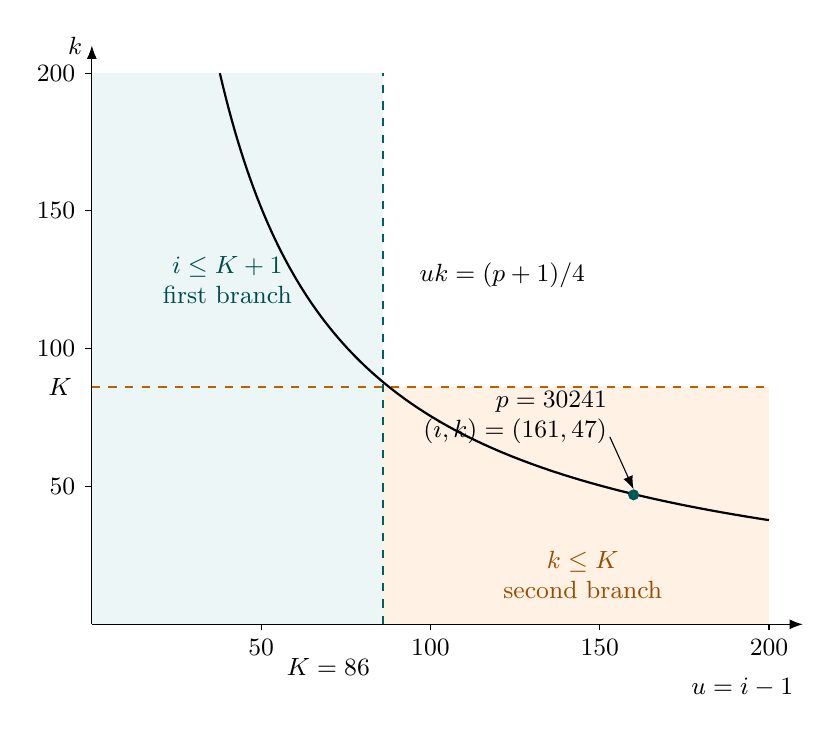
\begin{tikzpicture}[x=.043cm,y=.035cm,>=Latex,font=\small]
 \fill[teal!7] (0,0) rectangle (86,200);
 \fill[orange!10] (86,0) rectangle (200,86);
 \draw[->] (0,0)--(210,0);
 \node[anchor=north east] at (210,-16) {$u=i-1$};
 \draw[->] (0,0)--(0,210) node[left] {$k$};
 \foreach \x in {50,100,150,200}{
   \draw (\x,0)--(\x,-2) node[below] {\x};
   \draw (0,\x)--(-2,\x) node[left] {\x};
 }
 \draw[teal!75!black,dashed,thick] (86,0)--(86,200);
 \draw[orange!75!black,dashed,thick] (0,86)--(200,86);
 \draw[black,thick,domain=37.81:200,samples=180]
       plot (\x,{7560.5/\x});
 \node[anchor=south west,fill=white,inner sep=2pt] at (95,120)
       {$uk=(p+1)/4$};
 \node[align=center,text=teal!60!black] at (40,125)
       {$i\le K+1$\\first branch};
 \node[align=center,text=orange!60!black] at (145,18)
       {$k\le K$\\second branch};
 \fill[teal!70!black] (160,47) circle[radius=2pt];
 \draw[->] (153,68)--(160,49);
 \node[anchor=east,align=right] at (155,75)
       {$p=30241$\\$(i,k)=(161,47)$};
 \node[anchor=north east] at (85,-9) {$K=86$};
 \node[anchor=east] at (-3,86) {$K$};
\end{tikzpicture}
\end{document}
